\section{PnP}
\begin{itemize}
  \item \textbf{Got:} 2D-3D correspondences
  \item \textbf{Want:} $T, R$ between camera and world coordinate
    system.
\end{itemize}

\textbf{Solutions}
\begin{itemize}
  \item Linear hack
  \item Non-linear optimization
  \item P3P
\end{itemize}

\subsection*{P3P}
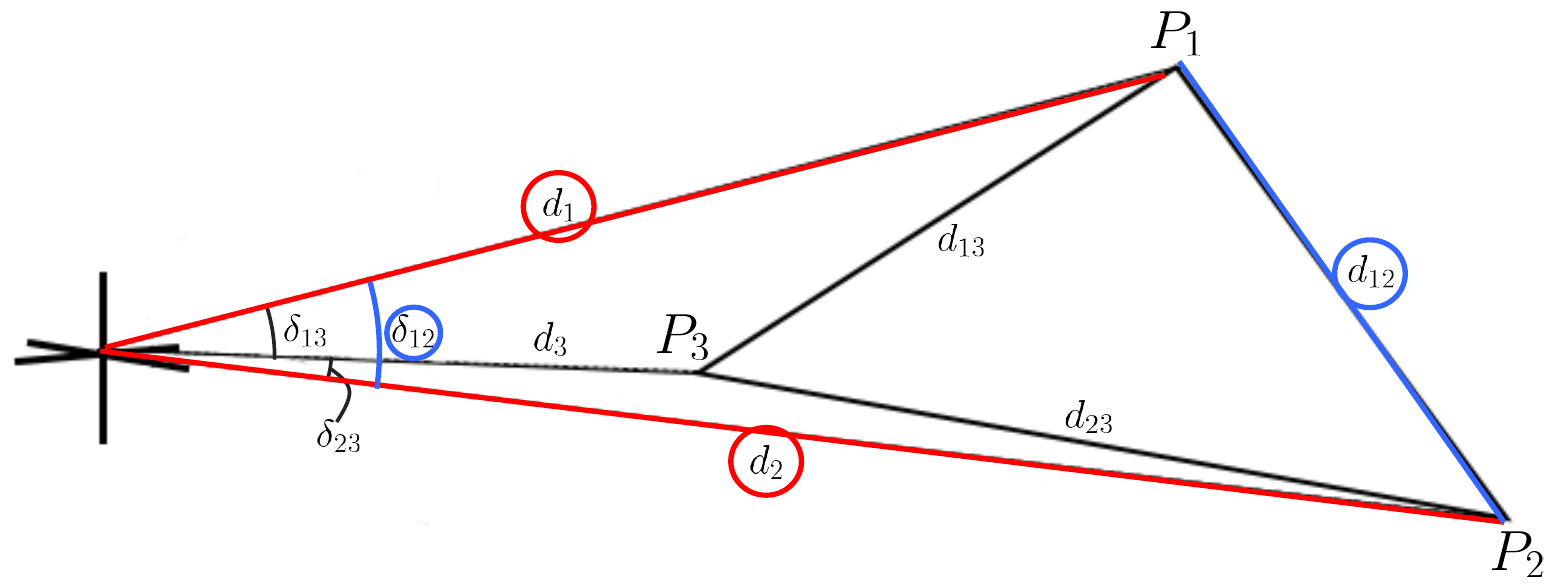
\includegraphics[width=\linewidth]{Images/P3P.png}
Simple formulation:\\
$d_i^2 + d_j^2 - 2 d_i d_j \cos(\delta_{ij}) = d_{ij}^2$\\
\alert{Use this for simple problems!}

Complex formulation: we use $d_2 = u d_1$, $d_3 = v d_1$, then:\\
$d_{13}^2 (u^2 + v^2 - 2 u v \cos(\delta_{23}) \\= 
d_{23}^2(1+v^2 - 2 v cos(\delta_{13}))$\\
$d_{12}^2 (1 + v^2 - 2v \cos(\delta_{13})) \\=
d_{13}^2 (1 + u^2 - 2u \cos(\delta_{12}))$
\begin{enumerate}
  \item Solve $u^2$ in 1.
  \item Insert $u^2$ back into 2.
  \item Solve $u$, leaving tems in $v$ and $v^2$.
  \item Insert $u$ back into 1. Quartic polynomial in $v$, at most 4
    solutions.
\end{enumerate}
